\chapter{State of the art}
This chapter will go through relevant articles and already known knowledge on the subject of mixed criticality systems, vehicle platooning and safety standards in the automotive industry.

\section{Mixed criticality systems}
%SotA regarding MCS.
A MCS is achieved by letting applications of different criticality share resources. These resources could be the processor, memory, peripherals, input/output ports etc. The most explored area is sharing the CPU between multiple criticality levels \cite{burns2016}. The benefit of combining previously distributed systems is higher resource efficiency, which leads to economical benefits.

%The term Mixed Criticality had been used before 2007 to address issues of non-interference in non-federated architectures such as IMA [190];

\subsection{Economical benefits of MCS}
%Lower production cost, higher design cost?
Potential benefits with pursuing MCS as opposed to distributed systems are reduced physical space required, reduced weight, reduced heat generation, reduced power consumption and reduced production costs~\cite{burns2016}. This would all ultimately lead to economical benefits.\\

Potential downsides are increased complexity which could lead to higher system design costs. Building applications on the same platform to share resources could require engineering teams to work more closely together, potentially leading to administrative difficulties and costs. This needs to be investigated and could vary from industry to industry. To combat the potential downsides, the EMC\textsuperscript{2} project aims at creating platforms for easier development of MCS.\\ %TODO: källa eller ändra wording

The EMC\textsuperscript{2} project lists several goals \cite{website:emc2goals}:
\begin{itemize}
\item Reduce the cost of the system design by 15\%
\item Reduce the effort and time required for re-validation and re-certification of systems after making changes by 15\%
\item Manage a complexity increase of 25\% with 10\% effort reduction
\item Achieve cross-sectorial reusability of Embedded Systems devices and architecture platforms that will be developed using the ARTEMIS JU results.
\end{itemize}

\subsection{Sharing processor}
%A lot of work has been done regarding processor scheduling in MCS
%TODO: Wording
To deal with many different tasks needing processor time, different schedulers can be used to appropriately distribute processor time among the tasks.

\subsubsection{Conventional scheduling}
The simplest scheduling algorithm is First In First Out (FIFO). As the name suggests, the first task to enter the queue is also executed first, and executes until it is finished~\cite{remzi2015}.\\

Another simple scheduling algorithm is Fixed Priority (FP). Each task is assigned a priority level, and the task with the highest priority in the queue is allowed to execute~\cite{liulayland1973}.\\

The scheduling algorithm Rate Monotonic (RM) assigns a priority level to a task depending on its frequency. Higher frequency leads to higher priority. The algorithm was proven optimal under the assumption that the deadline of every task coincided with its rate~\cite{liulayland1973}.\\

Deadline Monotonic (DM) assigns a priority level to a task depending on its deadline. Shorter deadline leads to higher priority~\cite{liulayland1973}.\\

Earliest Deadline First (EDF) is a dynamic scheduling algorithm that executes the task with the least amount of time left until its deadline.\\

Round Robin (RR) scheduling lets each task in the job queue execute for a predefined amount of time (called a time quanta), and if a task does not complete it is preempted and placed back in the queue waiting for its next time slot~\cite{kleinrock1964}.

\subsubsection{Mixed criticality scheduling}
The area of sharing the processor in MCS was first explored by Steve Vestal~\cite{vestal2007} in 2007. His paper showed that neither Rate Monotonic (RM) nor Deadline Monotonic (DM) priority assignment was optimal for MCS.% however Audsley’s optimal priority assignment algorithm \cite{audsley2001} was found to be applicable.\\ %TODO: Wording

In 2008 Baruah and Vestal~\cite{baruah2008} showed that EDF (Earliest Deadline First) does not dominate FP when criticality levels are introduced, and that there are feasible systems that cannot be scheduled by EDF.\\

%TODO: wording
One MCS scheduling algorithm is Criticality Monotonic Priority Ordering (CrMPO). Tasks are assigned priorities first according to criticality (highest criticality first) and then according to deadline (shortest deadline first). Static Mixed Criticality with no run-time monitoring (SMC-NO) is the scheduler that was Vestal's original approach~\cite{vestal2007}. Another scheduler is SMC with run-time monitoring (abbreviated only as SMC). Yet another scheduling algorithm is Adaptive Mixed Criticality (AMC), described Baruah, Burns and Davis~\cite{baruah2011}: "To summarise the main difference between SMC and AMC, in SMC any LO-critical task is descheduled if it executes for more than C(LO). While in AMC, all LO-critical tasks are descheduled if any job (from any task) executes for more than C(LO). If a HI-critical job executes for more than C(LO) (but no greater than C(HI)) then, under SMC, LO-critical tasks continue to execute but may miss their deadlines; but under AMC they stop executing."\\

To evaluate the performance of the different scheduling algorithms Baruah, Burns and Davis~\cite{baruah2011} tested the scheduling algorithms AMC, SMC and CrMPO for scheduling sporadic tasks of a taskset of 20 tasks where on average 50\% where of high criticality and 50\% where of low criticality. The tasks of high criticality where allowed an execution time that was twice its low criticality execution time. The comparison of the performance of the schedulers can be seen in Figure~\ref{fig:schedulers}. In the graph the UB-H\&L line bounds the maximum possible number of schedulable task sets.

%"This figure plots the percentage of task sets generated that were deemed schedulable for a system of 20 tasks, with on average 50\% of those tasks having high criticality and each task having a high criticality execution time that is twice its low criticality execution time. The compared approaches are (from least effective to most effective): CrMPO which assigned priorities in criticality order, SMC-NO (static  mixed criticality with no run-time  monitoring) which  is  Vestal’s  original approach, SMC which is an adaptation of Vestal’s approach in which LO-criticality tasks are monitored at run-time and are prevented from executing for more than C(LO), and AMC-rtb and AMC-max which are the two methods introduced in the previous paragraph (AMC for adaptive mixed criticality). In the graph the UB-H\&L line bounds the maximum possible number of schedulable task sets. It serves to illustrate the quality of the AMC-max approach."~\cite{burns2016}

\begin{figure}[H]
\centering
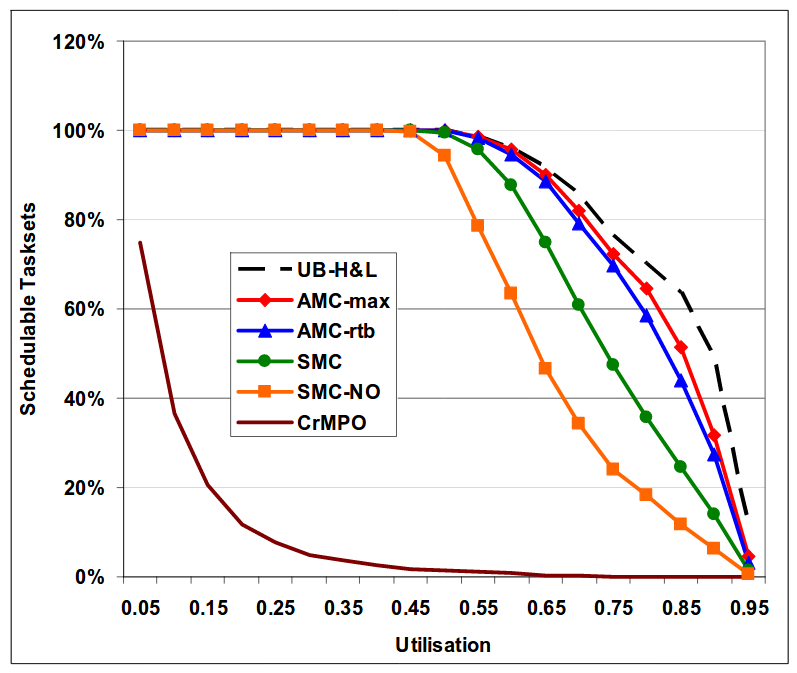
\includegraphics[width=\textwidth]{./img/literature_schedulers.png}
\caption{Percentage of schedulable tasks.~\cite{baruah2011}}\label{fig:schedulers}
\end{figure}

For a more complete review of work done on MCSs with a shared processor, see the paper by Burns~\cite{burns2016}.

%\subsection{Different criticality on different processors}


%\subsection{Sharing memory}
%http://pertsserver.cs.uiuc.edu/~mcaccamo/papers/euromicro12.pdf

\section{Standards}
%Different standards to regulate and ensure safety
Safety practices are becoming more regulated as industries adopt a standardized set of practices for designing and testing products. %TODO: expand, wording
To ensure safe and secure practices in industries, safety standards are becoming more regulated. Different standards address different areas. Below, the two safety standards IEC~61508 and ISO~26262 will be described.

\subsection{IEC 61508}
IEC 61508~\cite{IEC61508} is intended to be a basic functional safety standard for electrical and electronic systems applicable to all kinds of industry. It defines four different safety integrity levels, SIL~1 being the least dependable up to SIL~4 which is the most dependable level.

\subsection{ISO 26262}
ISO 26262~\cite{ISO26262} addresses the needs for an automotive-specific international standard that focuses on safety critical components. ISO 26262 is a derivative of IEC 61508.

\subsubsection{ASILs}
%ASIL QM (quality management) relates to the lowest (no) hazard, and ASIL
ISO 26262 describes five different Automotive Safety Integrity Levels (ASIL) relating to hazard and risk. Ranked from lowest (no) hazard to highest hazard, these levels are: QM, A, B, C and D. A function is assigned an ASIL depending on the severity if the function fails, the probability that the function fails and the controllability of the function, see table~\ref{table:ASIL}.

\begin{table}[H]
\centering
\begin{tabular}{|c|c|c|c|c|}
\hline
\multirow{2}{*}{\textbf{Severity}} &\multirow{2}{*}{\textbf{Probability}} &\multicolumn{3}{|c|}{\textbf{Controllability}} \\ \cline{3-5}
 & &C1 &C2 &C3 \\ \hline
\multirow{4}{*}{S1} & E1 & QM & QM & QM \\ \cline{2-5}
 & E2 & QM & QM & QM \\ \cline{2-5}
 & E3 & QM & QM & A \\ \cline{2-5}
 & E4 & QM & A & B \\ \hline
\multirow{4}{*}{S2} & E1 & QM & QM & QM \\ \cline{2-5}
 & E2 & QM & QM & A \\ \cline{2-5}
 & E3 & QM & A & B \\ \cline{2-5}
 & E4 & A & B & C \\ \hline
\multirow{4}{*}{S3} & E1 & QM & QM & A \\ \cline{2-5}
 & E2 & QM & A & B \\ \cline{2-5}
 & E3 & A & B & C \\ \cline{2-5}
 & E4 & B & C & D \\ \hline
\end{tabular}
\caption{ASIL as a function of severity, probability and controllability.}
\label{table:ASIL}
\end{table}

The various integrity levels can be translated into integers (ASIL $QM = 0$; $A = 1$; $B = 2$; $C = 3$ and $D = 4$). If a hazard requires several components to fail, the added ASIL of these components is used to determine if there is an violation, assuming the components faults are statistically independent of each other. For example, a safety level ASIL B can be met by two independent components which each individually only meet ASIL A (and thus effectively $A + A = B$).~\cite{azevedo2014} \\ %TODO: semi Wording

The different ASILs can relate to cost according to various cost heuristics, see table~\ref{table:cost_heuritics}. %TODO: Expand, wording

\begin{table}[H]
\centering
\begin{tabular}{|c|c|c|c|c|c|}
\hline
\textbf{Cost Heuristic} & \textbf{QM} & \textbf{A} & \textbf{B} & \textbf{C} & \textbf{D} \\ \hline
Linear & 0 & 10 & 20 & 30 & 40 \\ \hline
Logarithmic & 0 & 10 & 100 & 1000 & 10000 \\ \hline
Experimental-I~\cite{azevedo2014} & 0 & 10 & 20 & 40 & 50 \\ \hline
Experimental-II~\cite{azevedo2014} & 0 & 20 & 30 & 45 & 55 \\ \hline
\end{tabular}
\caption{ASIL cost heuristics.}
\label{table:cost_heuritics}
\end{table}


\subsubsection{Freedom from interference}
%TODO: Källa, utveckla, wording
In ISO 26262, Part 1, Definition 1.49, freedom from interference is defined as: Absence of cascading failures between two or more elements that could lead to the violation of a safety requirement. A cascading failure is defined as "failure of an element of an item causing another element or elements of the same item to fail" (ISO 26262, Part 1, Definition 1.13), and an element is defined as: "system or part of a system including components, hardware, software, hardware parts, and software units" (ISO 26262, Part 1, Definition 1.32)

\subsection{AUTOSAR}
%TODO: Wording
"AUTOSAR (AUTomotive Open System ARchitecture) is a international development partnership of automotive interested parties founded in 2003. It pursues the objective of creating and establishing an open and standardized software architecture for automotive electronic control units (ECUs) excluding infotainment. Goals include the scalability to different vehicle and platform variants, transferability of software, the consideration of availability and safety requirements, a collaboration between various partners, sustainable utilization of natural resources, maintainability throughout the whole "Product Life Cycle"."~\cite{website:autosar}\\

The AUTOSAR Architecture distinguishes on the highest abstraction level between three software layers: Application, Runtime Environment (RTE) and Basic Software (BSW) which run on a Microcontroller.~\cite{website:autosar} See figure \ref{fig:autosar}.
\begin{itemize}
\item The application software layer is mostly hardware independent.
\item The RTE represents the full interface for applications.
\item The BSW is divided in three major layers and Complex Drivers: Services, ECU Abstraction and Microcontroller Abstraction. Services are divided furthermore into functional groups representing the infrastructure for System, Memory and Communication Services.
\end{itemize}

\begin{figure}[H]
\centering
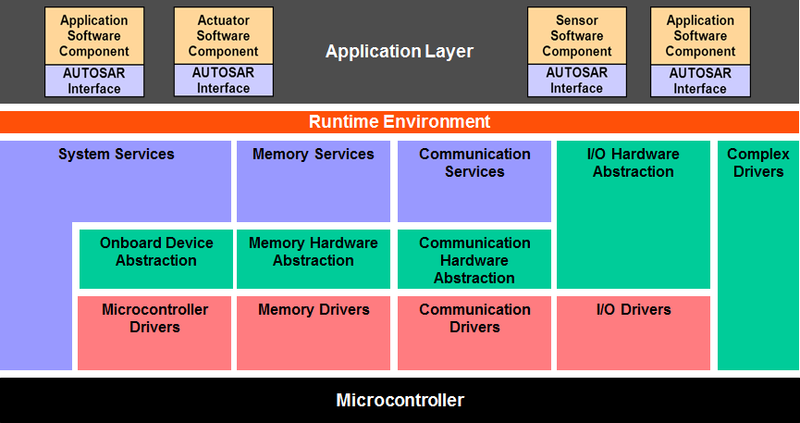
\includegraphics[width=\textwidth]{./img/literature_autosar.png}
\caption{AUTOSAR.~\cite{website:autosar}}\label{fig:autosar}
\end{figure}

\section{Hypervisors}
A virtual machine monitor, or hypervisor, can be seen as an interface between the operative systems and the hardware of a system. In order to facilitate for multiple operative systems of different criticality an appropriate hypervisor should be used. A system will only be as secure as its hypervisor, so it is important that the hypervisor has been engineered to at least the same standards as the most critical functions that will be implemented on the system. Other things to consider is that some hypervisors can accommodate multiple instances of operative systems, and some only facilitate for two. A description of a few available open-source hypervisors will follow.

\subsection{SafeG}
\label{sec:safeg}
SafeG is a hypervisor developed by the TOPPERS group of Nagoya University in Japan~\cite{website:safeg}. It can host two operating systems on the same hardware, partitioning them into Trusted and Non-Trusted zones (sometimes called Trusted and Non-Trusted "worlds") via ARM TrustZone~\cite{website:ARM}. This provides full system access to the software running in Trusted state, and limits the access and capabilities of the software running in Non-Trusted state.\\

Figure~\ref{fig:safeg} depicts the SafeG architecture. It shows a simplified view of a TrustZone enabled ARM processor together with partitioned memory and device IO.

\begin{figure}[H]
\centering
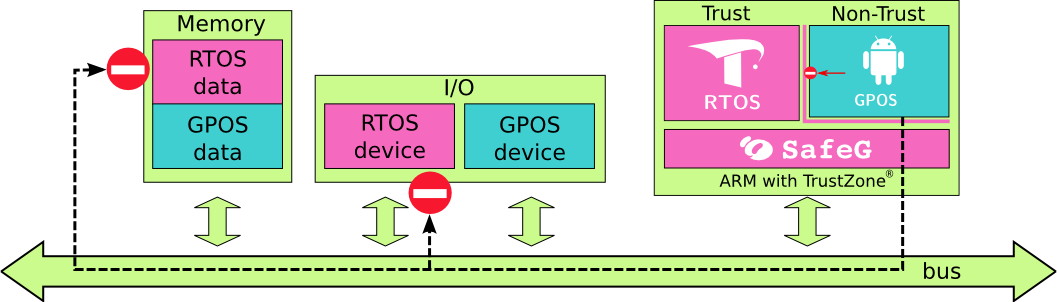
\includegraphics[width=\textwidth]{./img/literature_safeg.png}
\caption{SafeG and TrustZone.}\label{fig:safeg}
\end{figure}

The features of SafeG as described on their website are as follows~\cite{website:safeg}:

\begin{itemize}
\item Enables the concurrent execution of RTOS and GPOS on either single-core or multi-core ARM-based platforms.

\item Devices and memory regions that are configured as Secure are protected against illegal GPOS accesses.

\item Normal world devices can be accessed from both GPOS (Non-Trusted) and RTOS (Trusted) software.

\item Real-time requirements are guaranteed in RTOS (Trusted) via the utilization of FIQ and IRQ interrupts, where FIQ interrupts are issued for RTOS and IRQ interrupts are issued for GPOS. While in the Trusted state, IRQ interrupts are disabled so that GPOS can not disturb the execution of the RTOS. Therefore, GPOS only executes when the RTOS issues the Secure Monitor Call (SMC) instruction, which causes the SafeG monitor to switch from the Trusted world (RTOS) to the Non-Trusted world (GPOS). Furthermore, FIQ interrupts are active during the execution of GPOS, which enables RTOS to retake control of the system. For example, a cyclic execution of RTOS/GPOS can be controlled by an FIQ interrupt of a system timer.

\item GPOS does not require any major changes, and can execute with minimal overhead.

\item Includes an efficient guest-to-guest communication mechanism (i.e.referred to as SafeG COM).
\end{itemize}

The RTOS tasks are statically mapped to a processor during compilation, while the GPOS uses all available virtual CPUs in Symmetric Multi-Processor mode.\\

The SafeG Monitor is the gateway between the GPOS and the RTOS. During the switch operation, it is responsible for saving the state of one zone and loading the state of the other. According to TOPPERS~\cite{safegswitch}, the WCET of switching the OS is just under $2 \mu s$, see table~\ref{table:safegswitch}.

\begin{table}[H]
\centering
\begin{tabular}{|l|c|}
\hline
Switch path & WCET\\ \hline
Switch from RTOS to GPOS & $1.5 \mu s$\\ \hline
Switch from GPOS to RTOS & $1.7 \mu s$\\ \hline
\end{tabular}
\caption{WCET of switching OS.~\cite{safegswitch}}
\label{table:safegswitch}
\end{table}

\subsection{SICS Thin hypervisor}
SICS Thin Hypervisor (STH) is a light-weight hypervisor designed for ARM-based devices~\cite{STH2013}. STH runs directly on top of the hardware (bare metal), and achieves system virtualization through paravirtualization. STH allows for more than two guests to run on top of the hypervisor.\\

There is no graphical support and all communication with the kernel is done through the UART.\\

The current version of STH supports ARMv5 (926EJ-S) and ARMv7 Cortex-A8 only, but due to its flexible nature and minimal layer of hardware abstraction it is easily migrated to other platform~\cite{STH2013}.

\subsection{Sierra visor}
Sierraware offers a bare metal universal hypervisor (SierraVisor) that is
available as open-source under the GNU GPL v2 license or with a commercial
license [33]. It supports paravirtualization, TrustZone virtualization, and
hardware assisted virtualization. SierraVisor is compatible with Cortex-
A9/A15 and ARM11 based SoCs, but only Cortex-A15 supports the
hardware assisted virtualization option * . The TrustZone virtualization
approach allows for the integration of guest operating systems without any
kernel modifications. Each guest kernel and applications run in their usual
privilege mode, supervisor and user mode respectively. Furthermore, each
guest executes in an isolated container with low overhead.

\subsection{Xen hypervisor}
The Xen hypervisor is widely used in enterprise and is now making its way
to embedded systems. It was developed in Cambridge University, and is
available as open-source software under the the general public license (GNU).
The Xen hypervisor is implemented as the guest console architecture, as
discussed in subsection 4.2.4. The hypervisor layer is a thin software layer
that resides above the hardware layer. It is the first program that runs
after the bootloader, and is responsible for managing the CPU, Memory, and
interrupts.
By default, the Xen hypervisor uses Credit as the CPU scheduler, which
allows the user to allocate a percentage of the CPU time for each VM, or allow
the hypervisor to automatically balance the workload across active CPUs in
the system. Alternatively, the user can specify Simple Earliest Deadline First
(SEDF) algorithm for the scheduler. However, the load-balancing feature will
be unavailable [28].
The hypervisor is responsible for launches Dom0, which is a special virtual
machine that has privileged access rights to the physical I/O resources. It
handles I/O accesses and interacts with the other virtual machines. All other
VM instances operate in Domain U (DomU), which runs in unprivileged mode. The guest virtual machines can be either paravirtualized (PV) or
fully virtualized {a.k.a. Hardware-assisted Virtual Machine (HVM)}. The
PV guest are modified operating systems such as: Linux, Solaris, FreeBSD,
or other UNIX operating systems. In order to facilitate I/O sharing, Xen
uses split-driver architecture. This approach manges I/O accesses of DomU
PV guests. The split-driver technique divides the driver into a front-end,
located in the DomU PV guest, and a back-end, located in the Dom0 guest.
DomU PV guests are aware that they do not have direct access to the
hardware and that they are running alongside other virtual machines on the
same hardware. However, DomU HVM guests are unaware of the presence
of other VMs, and of the fact that they are sharing hardware resources.
Instead of split-drivers, in the HVM architecture, a special daemon is started
in Dom0 guest for each DomU HVM guest. The Xen hypervisor is available
for both Intel and ARM devices. However, it is not recommended to use Xen
with devices that do not contain IOMMU units because the hypervisor can
be easily subverted by DMA capable devices [29].

\subsection{Xen zynq}
The open-source Xen hypervisor has recently been ported to the new
Xilinx Zynq Ultrascale+Multi-Processor System-on-Chip (MPSoC) device
[30]. Xen Zynq Distribution is released under the GNU General Purpose
License 2 (GPL2). The processing platform features a quad-core ARM
Cortex-A53, a dual-core ARM Cortex-R5, a Mali-400MP2 GPU, and FPGA
fabric that supports run-time reconfiguration. This device is the successor of
Xilinx Zynq SoC, which features a dual-core Cortex-A9 processor and FPGA
fabric.

\subsection{SEL4 microkernel}
The sel4 microkernel is based on the L4 microkernel, which is one of the
smallest kernels available today. Sel4 is the first formally verified microkernel,
which implies that its specification is verified mathematically. Sel follows
the ”minimality principle”, which dictates that the kernel shall only contain
functionalities that can not be implemented at the user-level [31]. As a result,
the microkernel is small, efficient, and robust. All device drivers are excluded
from the microkernel level and execute in unprivileged mode, except for a
timer driver and an interrupt controller driver.
The microkernel supports a small number of services that enable applicationsto create and manage threads, virtual memory spaces, and interprocess
communication (IPC). Furthermore, sel4 follows a ”capability-based access
control model” in order to manage the access rights to all kernel services.
Capabilities are unforgeable tokens that contain metadata about a specific
kernel object, including its access rights. The use of capabilities as a control
mechanism allows the system to maintain strong isolation between software
components [32].
The sel4 microkernel implements a fixed-priority round-robin scheduler
policy, mainly because its current ”time” abstraction method is under-
developed and does not yield satisfactory results. As proposed in [31],
reservations can be added to sel4 in order to provide a suitable temporal
isolation solution for real-time systems.
Sel4 provides IOMMU support for Intel-based architectures (IA-32),
which allows the safe integration of DMA enabled devices. Furthermore,
Sel4 can support multicore systems via multikernel bootstrapping. However,
this feature is only available for x86 machines; only uniprocessor is supported
for ARM-based devices.

\section{Field Programmable Gate Array}
%FPGA sota
%TODO: some wording, probably longer
A Field Programmable Gate Array (FPGA) is an array of logic gates with reconfigurable interconnects that can be connected to each other. As the name suggests, it is possible to reprogram the physical function of the FPGA "in the field". This is what distinguishes a FPGA from an Application Specific Integrated Circuit (ASIC), an ASIC can not be reprogrammed after manufacturing.\\ %Generally, ASICs have slightly higher performance and are cheaper to produce in higher quantities.

To program the behavior of the FPGA, Hardware Descriptive Language (HDL) is used. The two most widely used HDLs are Verilog and VHDL (VHSIC Hardware Descriptive Language, where VHSIC is an acronym for Very High Speed Integrated Circuit)~\cite{DO178C}. Verilog came to existence late 1983. The language was standardized as IEEE standard 1364-1995, and has since been revised and included in IEC/IEEE Behavioural Languages standard 61691~\cite{IEEEVerilog}. Work with VHDL formally began in 1981, and in 1987 it was standardized as IEEE-1076. The active standard for VHDL is also part of the IEC/IEEE Behavioural Languages standard 61691~\cite{IEEEVHDL}. Using Google Trends~\cite{googletrends} with the search terms "vhdl" and "verilog", one can see that Verilog seems to be the more popular language of the two in the USA, India and South Korea, while VHDL is more used in Europe and South America, see Figure~\ref{fig:vhdlverilog}.

\begin{figure}[H]
\centering
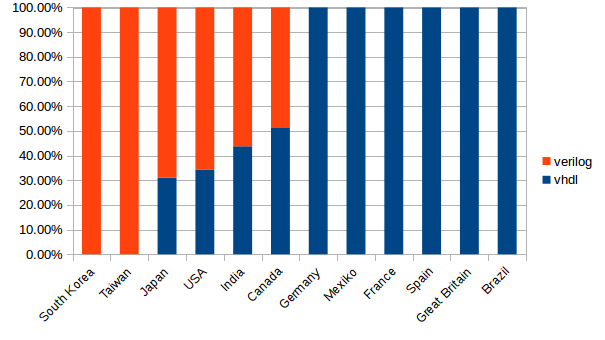
\includegraphics[width=\textwidth]{./img/vhdlverilog.png}
\caption{Distribution of Google searches for "verilog" vs "vhdl" in the world.}\label{fig:vhdlverilog}
\end{figure}

A key difference between code running on a processor and code describing functions in a FPGA is that traditional code is executed in serial, where only one computation can be executed at any one time. In a FPGA however, functions can run in parallel. This makes FPGAs excellent for implementation of hardware functions that require high speed and high frequency that you do not want to take up precious processor time.\\

Some FPGA circuits have non-volatile memory from where the hardware descriptive language is loaded when the circuit is powered up, this means that its configuration is not lost if its power goes down.

\section{Platooning}
%TODO: wording
Platooning, road trains or convoy driving is the concept of a chain of vehicles with no physical connection traveling at a given (short) intermediate distance in order to utilize the reduced air friction behind the vehicle in front. The primary objective for each vehicle with respect to safety is to maintain its distance to the preceding vehicle in the platoon.

\subsection{Benefits of platooning}
%TODO: Expand, wording, source
Potential benefits of vehicle platooning includes lower fuel consumption, less road space required and more efficient traffic flow.\\ 

Using simulations of platooning, Alam, Gattami, and Johansson \cite{johansson2010} showed in 2010 that there is a \mbox{4.7--7.7\%} fuel reduction potential in heavy duty vehicle platooning at a set speed of 70 km/h with two identical trucks.\\

In 2014, Lammert et. al.~\cite{lammert2014} showed in tests that platooning can result in reduced fuel consumption of up to 5.3\% for the lead vehicle and up to 9.7\% for following vehicles.\\

Tests by truck manufacturer Scania have shown that platooning can reduce fuel consumption by up to 12\%~\cite{scania2015}.

\subsection{Safety requirements for platooning}
%TODO: more sources
With shorter distance between vehicles, the margin of error also decreases. This puts high requirements on the system controlling the speed of the vehicles in the platoon.\\

In the article by Alam et al.~\cite{johansson2013}, safe sets for heavy duty vehicle platooning are computed to calculate minimum distance between the  vehicles in a platoon without endangering safety. System uncertainties or varying vehicle parameters, such as mass, air resistance and road gradient, could cause a difference in braking capabilities between the vehicles, thereby changing the shape of the safe sets. If the follower vehicle has a higher braking capacity, it will be able to lie closer without endangering a collision. The minimum safe relative distance is therefore shorter compared to the case of two identical vehicles. However, if the lead vehicle has a greater braking capability the relative distance must be increased significantly. Delays for the platoon control system commonly occur due to detection, transmission, computation, and producing the control command. A delay in the system implies that the lead vehicle will be able to act, change the relative velocity and distance, before the follower vehicle is able to react. A delay can be translated into a shift of the reachable set. However, no change occurs in the follower vehicle's velocity, since it does not react. Depending on the radar and the collision detection algorithm, a worst-case delay is approximately 500~ms for the considered vehicles. Hence, the lead vehicle will be able to reduce the relative velocity by 3.25~m/s and the relative distance by 0.8~m if it is driving 25~m/s at normal mode. Thus if the follower vehicle maintains a distance of at least 2~m, a collision can always be avoided for two identical vehicles~\cite{johansson2013}.

%\section{Lane detection and lateral control}
